\chapter{Contexte et besoin}
\section{Mon rôle au CEA}
Le CEA (Commissariat à l’Énergie Atomique et aux Énergies Alternatives) est un établissement public industriel et commercial (EPIC) de droit privé. Ce statut lui permet d’avoir des activités avec différentes sociétés privées ou publiques tout en étant financé par l’état français. Le CEA a été créé en 1945 sous l’ordonnance du général Charles De Gaulle. Il a pour but de réaliser les recherches sur le nucléaire et d’acquérir la maîtrise de l’atome. Il intervient ainsi dans quatre grands domaines de recherche : la défense, les énergies décarbonées, les technologies pour l’information et la santé, et la recherche fondamentale. 

C’est en 1946 que le site de Gramat, situé au sein du parc naturel régional des causses du Quercy dans le Lot, est retenu pour implanter, dans le gouffre de Bèdes, des bancs d’essais de propulseurs de grande puissance (V2). En 1956, le site devient le polygone d’expérimentations de la section atomique de la DEFA (Direction des Études et Fabrication d’Armement) et accueille les premiers essais liés au fonctionnement détonique des armes nucléaires. En 1959, le site devient le CEG (Centre d’Etudes de Gramat), dépendant de la DGA (Délégation Générale pour l’Armement), puis, en 1965, les essais liés au fonctionnement détonique (non nucléaire) de l’arme nucléaire commencent. En 1965, des essais sur la dynamique des roches et les études de durcissement électromagnétique et mécanique sont mis en place. C’est en janvier 2010 que le CEG de la DGA a rejoint le CEA. Il devient ainsi le dixième centre du CEA et le cinquième centre de la DAM. Le site s’étend aujourd’hui sur 325 hectares et emploie 260 salariés ainsi que des stagiaires, apprentis et thésards. Il est le centre de référence pour l’étude de l’efficacité des armements et de la vulnérabilité des systèmes aux effets des armes conventionnelles et nucléaires. Il dispose de nombreux moyen expérimentaux comme le lanceur Ares présenté en figure \ref{ares}, qui permet de mesurer le comportement de matériaux soumis à des agressions physique extrêmes.

\begin{figure}[h]
\centering
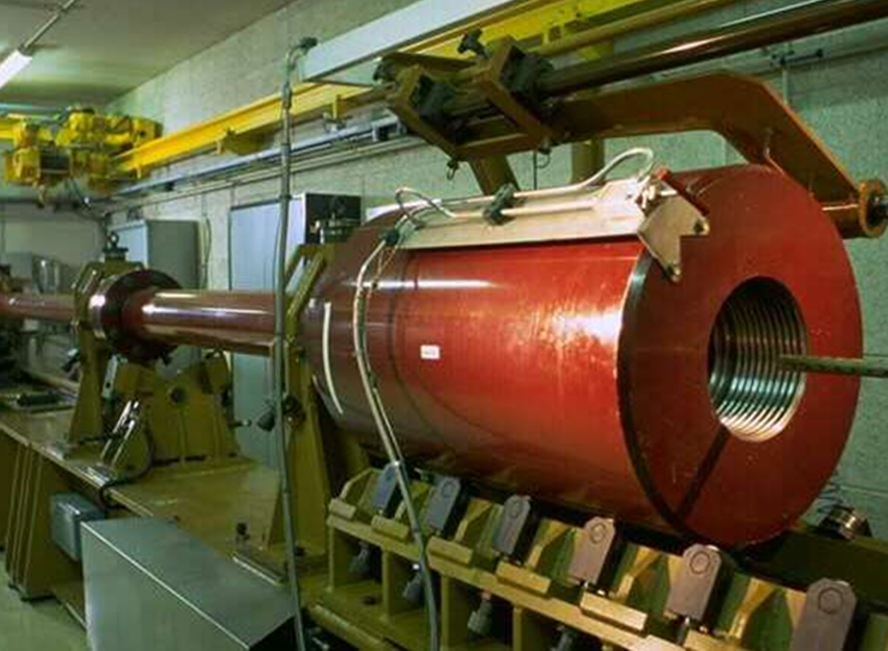
\includegraphics[scale=0.5]{ares.png}
\caption{Lanceur Arés} 
\label{ares}
\end{figure}

Dans le cadre de mon alternance, suis intégré dans le Service Détonique, Mécanique et Thermique (SDMT) au Laboratoire Détonique et Thermique (LDT).

La majorité des travaux du LDT portent sur la détonique. Il y a donc un fort besoin en applications spécifiques afin de répondre à des problématiques liées à la recherche. De nombreux logiciels sont développés en interne afin d'être au plus proche du besoin. Mon rôle est donc d'améliorer ces logiciels internes ou d'en développer des nouveaux. Je peux ainsi être amené à intervenir sur différentes étapes d'un projet, ou bien être responsable de l'intégralité d'un projet. 

\newpage

\section{Description de Siame}

Le centre d'étude dispose de nombreux codes de calcul et de simulation. Un de ces codes, Siame (SImulation Aérothermochimique de la Mécanique des Explosifs), a été principalement développé au laboratoire afin de répondre à des problématiques de défense. Il permet notamment d’obtenir des informations sur la composition et le comportement réactif d’un mélange de matériaux énergétiques dans un contexte thermodynamique. Ces informations peuvent par la suite être utilisées dans d’autre code de simulation pour décrire le comportement de différents matériaux. Siame est principalement utilisé par le CEA ainsi que par différents acteurs de la défense française. Une capture d’écran de l’IHM de Siame est présentée en figure \ref{screen}.

\begin{figure}[h]
\centering
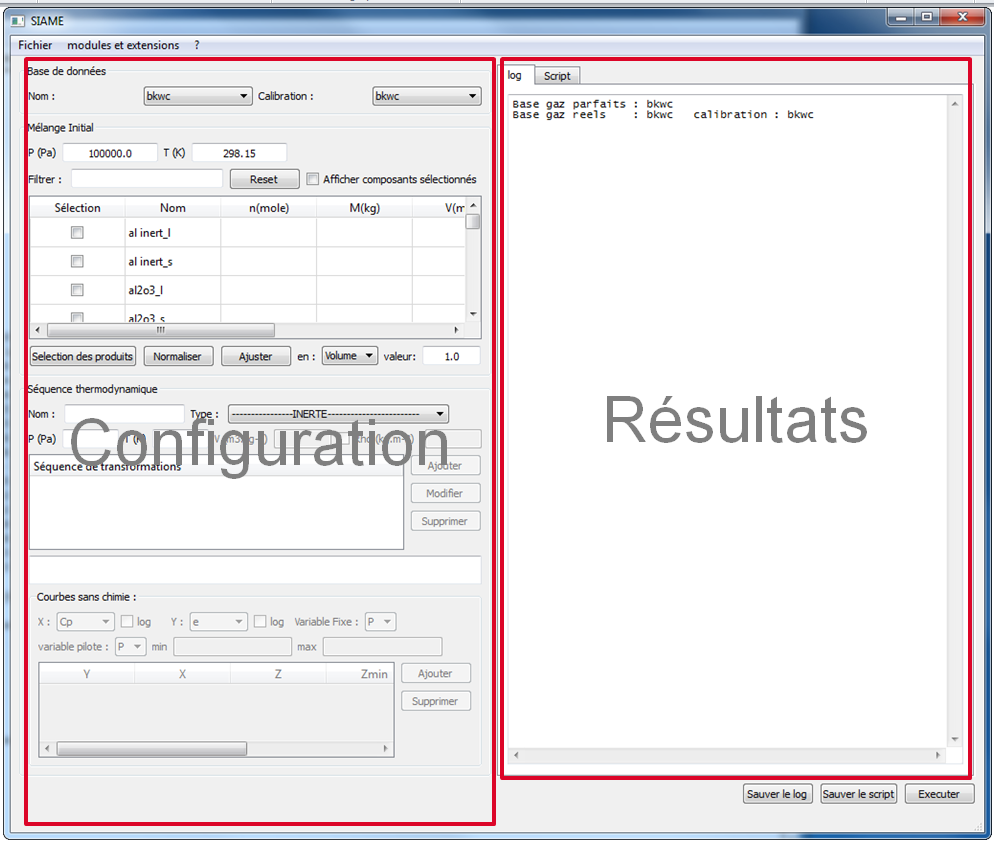
\includegraphics[scale=0.5]{Siame.png}
\caption{IHM de Siame} 
\label{screen}
\end{figure}

Siame est un programme écrit en plusieurs langages, principalement Python et Fortran. Ceci permet de combiner la flexibilité du Python avec la vitesse du Fortran. L'architecture très particulière de Siame sera détaillée ultérieurement. 

\begin{figure}[h]
\centering
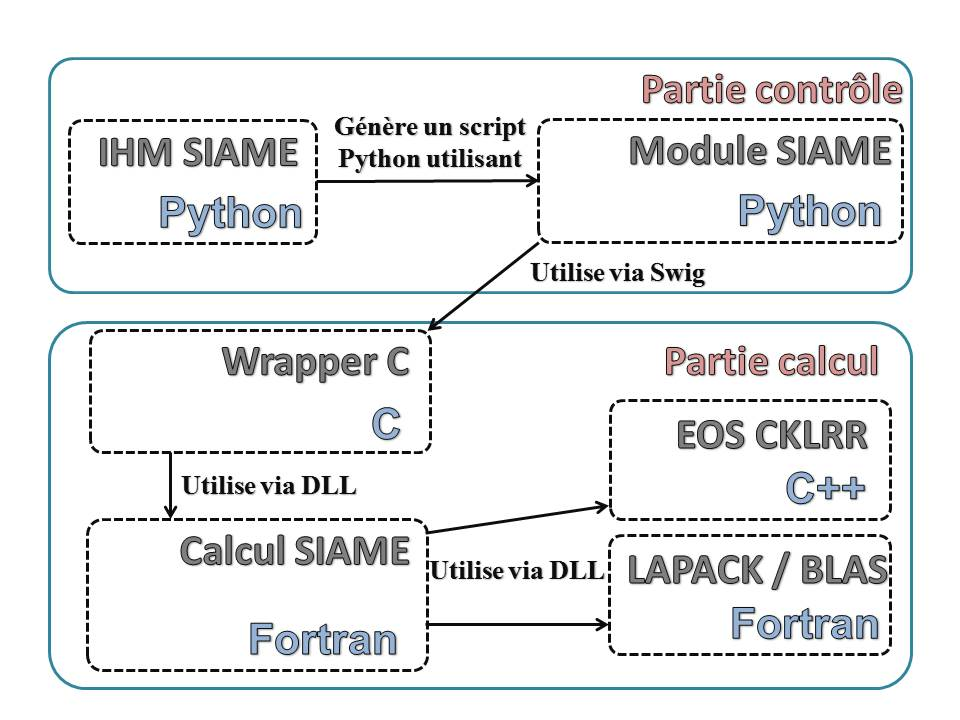
\includegraphics[scale=0.5]{SiameFonct.jpg}
\caption{Architecture de Siame} 
\label{archi}
\end{figure}

L'architecture si particulière est une des raisons principale pour lesquelles un sous-traitant est intervenu pour une partie du développement. Ce travail portera sur la façon dont a été gérée cette sous-traitance.

Les principales personnes qui ont été impliquées dans le projet sont Marc Genetier (Ingénieur Chercheur), Gérard Baudin (Ingénieur Chercheur) et Brigitte Martegoutte (Gestion des achats). Les dates, nom d'entreprises et montants ne sont donnés qu'à titre indicatif. 

\section{Besoin en sous-traitance}

Comme vu dans la partie précédente, l'architecture de Siame est particulière. Les domaines d'expertise du laboratoire étant en détonique, la mise en place de ce type d’architecture n’est pas dans les missions premières du LDT. Une maquette intégrant la partie thermochimique du code a été développé en interne, et il a été décidé de sous-traiter la mise en place de l'architecture présentée en figure \ref{archi}.

Ce choix est tout à fait justifiable puisque la mise en place d'une architecture complexe est un problème purement informatique. La partie la plus \og développement logiciel \fg{} a été sous traitée afin de permettre aux chercheurs de se concentrer sur la partie physique et scientifique du problème. 

La partie maquette / preuve de concept a été réalisée en amont par les chercheurs du LDT, expert du domaine. La partie industrialisation / mise en place de l’architecture est sous traitée afin de profiter des compétences d’entreprises spécialisées dans le développement d’applications scientifique. Une fois la version industrialisée opérationnelle, les chercheurs peuvent se servir de cette nouvelle version plus performante et y ajouter de nouvelles fonctionnalités. 

\chapter{Gestion du projet}

Le tableau \ref{chrono} présente une frise chronologique résumant les points clefs de la sous-traitance. 

\begin{table}[h]
\caption{Frise chronologique}
\label{chrono}
\centering
\begin{minipage}[t]{.7\linewidth}
\color{gray}
\rule{\linewidth}{1pt}
\ytl{01/13}{État des lieux codes de thermochimie}{teal}
\ytl{03/13}{Début du développement de la maquette}{teal}
\ytl{04/14}{Limites de la maquette atteinte}{teal}

\ytl{05/14}{Lancement d'appel à la concurrence}{cyan}
\ytl{06/14}{Début des négociations}{cyan}
\ytl{09/14}{Fin des négociations : Dev101 remporte le marché}{cyan}

\ytl{12/14}{1\textsuperscript{ére} livraison}{blue}
\ytl{05/15}{2\textsuperscript{éme} livraison}{blue}
\ytl{07/15}{3\textsuperscript{éme} livraison}{blue}
\ytl{08/15}{4\textsuperscript{éme} livraison}{blue}
\ytl{09/15}{5\textsuperscript{éme} livraison}{blue}
\ytl{10/15}{Fin du développement et début utilisation}{blue}

\ytl{10/16}{Fin garantie}{violet}

\rule{\linewidth}{1pt}%
\end{minipage}%
\end{table}


\section{Les débuts du projet}

Le projet Siame à commencer à voir le jour en début d'année 2013 avec un état des lieux des codes de thermochimie. Le principal programme répondant aux besoins du CEA est un code de thermochimie américain de nom de Cheetah. Ce programme présente cependant plusieurs défauts, notamment le fait qu'il soit impossible de le modifier ou de rédiger les simulations sous forme de script. Il n'a donc pas été jugé suffisant pour les besoins de la défense. La décision a alors été prise de développer un code de thermochimie français, du nom de Siame.

Siame a tout d'abord été écrit en Python comme une preuve de concept. Le développement de cette maquette s'est terminé début 2014 lorsque les temps de calculs sont devenus beaucoup trop longs. Le fait que la maquette montrerait ses limites et que le passage à un langage plus adapté serait nécessaire a toujours été prévu et il a été décidé de sous traiter ce changement. 

Le CEA est un pouvoir adjudicateur de la commande publique. Cela signifie qu'il est habilité à passer des marchés au nom de l'état. Les marchés entre 40 000 et 214 000€ sont donc publiés sur un site spécialisé accessible au grand public. Les principes qui régissent ces marchés sont le libre accès à la demande (offres en libre accès), la transparence (communiquer sur les raisons qui entrainent le rejet d'une offre) et l'égalité de traitement entre les concurrents (accès aux mêmes informations).


Un avis d’appel public à la concurrence a donc été publié en ligne. Ce document présente de manière succincte le besoin et spécifie principalement les modalités de candidature. On y apprend par exemple que le CEA accorde une grande importance à la capacité financière des entreprises partenaires. Des extraits de bilan des trois dernières années et le chiffre d’affaires sont demandés aux candidats et comptent pour une part importante de l’attribution de marché. 

Un cahier des charges de 18 pages est aussi publié afin de spécifier le besoin et clarifier le résultat attendu. On y trouve d’une part des informations sur le côté scientifique du projet comme le principe d’un code de thermochimie et des détails quant aux différents modèles à utiliser. On y retrouve aussi des points plus techniques comme les systèmes d’exploitation sous lesquelles la solution doit fonctionner ou des détails de l’IHM. Il présente pour finir des points de gestion de projets comme les exigences de garantie de la part du CEA, les modalités d’appréciation des livrables fourni par le sous-traitant ou encore les jalons clefs.


Le CEA exige que le projet soit facturé de manière forfaitaire et non pas au prorata du temps passé et qu'il soit composé d’une tranche ferme et de tranche optionnelle. La tranche ferme est composée d’une version fonctionnelle et assez complète des fonctionnalités de la maquette. Elle permet de faire toutes les simulations importantes et d’être interfacable avec d’autres applications. Un schéma décrivant les différentes fonctions de la tranche ferme est présenté en figure \ref{ferme}. La tranche optionnelle contient notamment des possibilités de simulations plus avancées et une IHM. 

\begin{figure}[h]
\centering
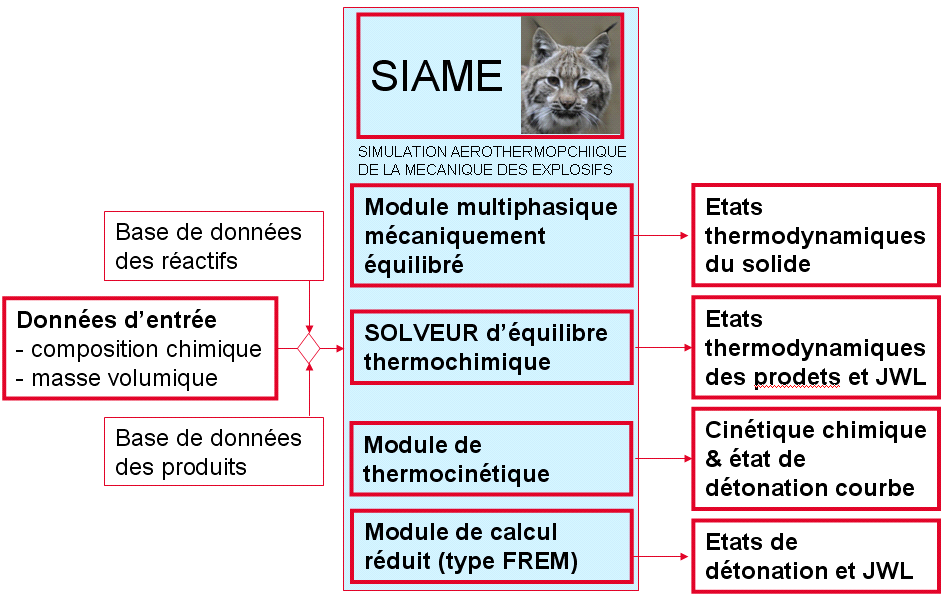
\includegraphics[scale=0.5]{siame_cahier_ext.png}
\caption{Description de la tranche ferme} 
\label{ferme}
\end{figure}

Le service des achats a publié la demande en mai 2014 et s'est occupé de la réception des candidatures.

\section{La gestion de la sous-traitance}
 
 Au total, 5 entreprises ont été intéressées par l'appel d'offre initial. Elles sont toutes des entreprises de taille considérable spécialisée dans le développement logiciel. Au final seul deux d'entre elles ont fait une offre, Dev202 et Dev101. Des réunions de négociation ont ensuite été réalisées afin de préciser le besoin et de discuter du prix. Le résultat de ces négociations peut être trouvé dans le tableau \ref{ref_prix} 
 
\begin{table}[h]
\caption{Récapitulatif des couts}
\label{ref_prix}
\begin{tabular}{l|lll|lll}
              &  \multicolumn{3}{c}{Dev101}       & \multicolumn{3}{c}{Dev202}               \\
             Tranche &  Ferme &  Optionnelle & Total &  Ferme & Optionnelle & Total \\
              \hline
Tarif initial (€) & 74358        & 42300             & 116658   &      83550         &      39094 & 122644 \\
Tarif négocié (€) &         59613     &        37737            &   97350    &      85627         &        37705            &      123332
\end{tabular}
\end{table}

L'entreprise Dev101 a remporté le marché car moins onéreuse pour une prestation similaire. Le cout total du projet est d’environ 100 000€ car la tranche fixe et la tranche optionelle ont été retenues.

Le CEA a accompagné Dev101 dans le développement de l’application. La mise à disposition de la preuve de concept leur a permis d’avoir une idée du résultat attendu et la preuve que ce résultat est atteignable. Beaucoup de documentation scientifique pertinente a été fourni afin que Dev101 puisse s’approprier la problématique. Des présentations ont été faites afin de spécifier dans les détails les méthodes de résolution appropriées. Une diapositive d’une des réunions de lancement est présentée figure \ref{reu_lancement}. On peut y voir le parallèle entre les différentes étapes de la simulation et le résultat attendu.

\begin{figure}[h]
\centering
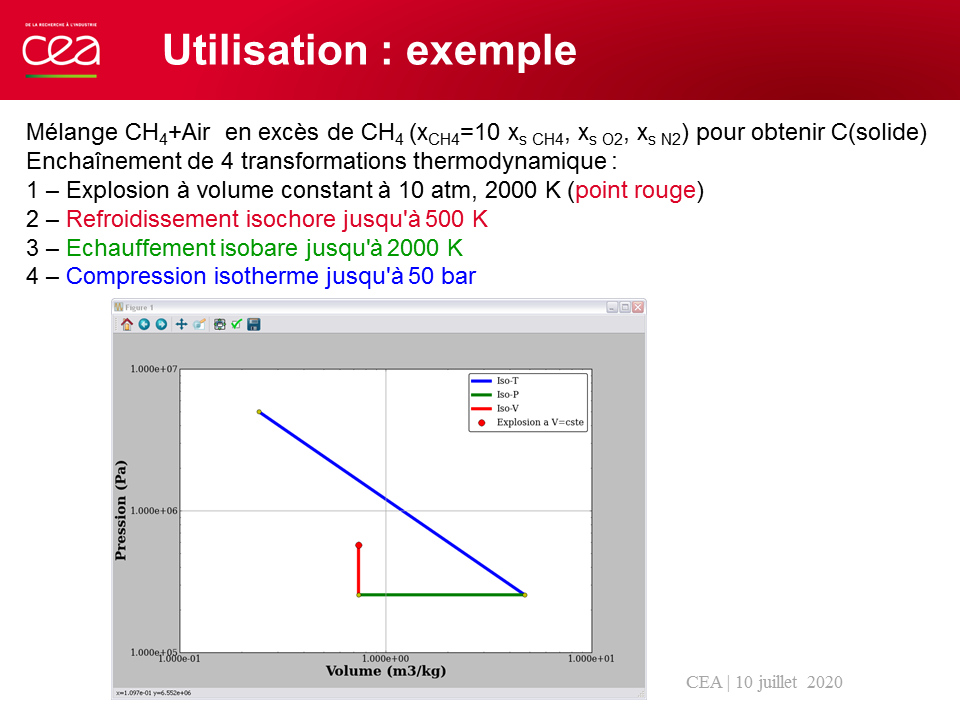
\includegraphics[scale=0.5]{demo_maquette.png}
\caption{Exemple résultat attendu} 
\label{reu_lancement}
\end{figure}

Dev101 à ensuite pu commencer à développer la solution et à la livrer. Au total 5 livraisons ont été effectuées sur un peu moins d’un an. Voici une description rapide de ce que contient chaque livraison : 
\begin{enumerate}
\item Implantation du noyau principal (19 656€) ;
\item implantation équation d’état (39 957€) ;
\item IHM (10 359€) ;
\item fonctionnalités supplémentaires (17 758€) ;
\item optimisation et portage (9 619€).
\end{enumerate}

Chaque livraison est suivie d’une courte phase de vérification. Durant cette phase, les membres du laboratoire peuvent tester le livrable, afin de vérifier qu’il est fonctionnel et correspond à la demande. Si ce n’est pas le cas, il est possible durant le mois suivant sa livraison, de signaler le problème à Dev101 afin que des corrections soient apportées.

Une fois la dernière livraison effectuée, une garantie d’un an commence. Cette garantie octroie un temps relativement long afin de détecter d’éventuels bugs et de les faire corriger. 5\%  du cout du projet est retenu jusqu'à la fin de cette garantie. Une fois la garantie expirée, le projet est considéré comme terminé et le solde de 5\% est payé au sous-traitant.

\section{Rétrospective}

Le projet s'est dans l'ensemble bien déroulé et toute les parties concernées sont satisfaites. Tous les livrables sont fonctionnels et ont été produit dans des temps raisonnables. Cette réussite est en partie le fruit de l'étroite collaboration entre le CEA et Dev101 au cours du projet.

Ce TR m’a permis de m’intéresser à la gestion d’un projet d’un point de vue assez différent de celui dont j'ai l'habitude. J’ai pu voir les différents acteurs ainsi que les procédures qui sont mise en place au CEA pour sous-traiter des développements. Ceci m'a permis de voir la démarche mise en œuvre pour lancer un appel d'offre, sélectionner le prestataire le plus adapté et encadrer le déroulement du projet.




